\chapter{$t\to qX$ analysis overview}
\label{chapter:tqXanalysis}

Flavour-changing neutral-currents (FCNC) interactions are not present at three level in the \acrshort{SMlabel} and are strongly suppressed at higher orders. Within the \acrshort{SMlabel}, the FCNC decay branching fraction of the top-quark into a Higgs boson, $t\to qH$ ($q=u,c$), is below 10$^{-15}$ well out of reach of sensitivity of the \acrshort{LHClabel}. Hence, any observation of such FCNC decays would be a direct sign of new physics.\\

The~\acrshort{ATLASlabel} and CMS collaborations have searched for various FCNC processes involving the top-quark and light-quarks, $q=u,c$ in $pp$ collisions at $\sqrt{s}$=7, 8 and 13~TeV with data samples ranging from 5.0 to 139 fb$^{-1}$, probing the top-quark decaying into photons $t\to q\gamma$~\cite{ATLAStqgamma,tqgamma2020,CMStqgamma,Tumasyan_2022}, into the $Z$ boson $t\to qZ$~\cite{Sirunyan_2017,tqZ2018,ATLAS-CONF-2021-049,CMStqZ}, into the Higgs boson $t\to qH$~\cite{ATLAStqHtautau,TOPQ-2017-07,CMStqHRun2,Khachatryan_2017}, and also in single top-quark production $q+g\to t$~\cite{tqgluon2016,tqgluon2021,tqgluon2017CMS}. Searches for similar signatures involving a FCNC decay of the top-quark into a beyond-the-SM particle lighter than the top-quark are uncovered in literature.\\

The analysis presented in this thesis is a search for a light scalar $X$ ($m_X < m_\text{top}$) in the $t\to qX$ decay\footnote{The process is denoted as $t\to qX$, with the charge-conjugate process $\bar{t}\to\bar{q}X$ implied.}, with $X\to\bbar$, performed with the full Run~2 proton-proton collision data of 139 fb$^{-1}$ at $\sqrt{s}$=13~TeV. The results of this search are public~\cite{ATLAS:2023mcc}:

\begin{itemize}
    \item ATLAS Collaboration, \textit{Search for a new scalar resonance in flavour-changing neutral-current top-quark decays $t\to qX$ $(q=u,c)$, with $X\to\bbar$, in proton-proton collisions at $\sqrt{s}$=13~TeV with the ATLAS detector}, arXiv:2301.03902

\end{itemize}

This chapter describes the $t\to qX$ analysis motivation, challenges and strategy. After a short introduction, the event selection is presented followed by the description of the modelling of the signal and background processes. Then, the analysis strategy and a summary of the systematic uncertainties are given. This analysis shares the methodology of the $H^+\to tb$ search presented in the previous part of the thesis and for the sake of brevity, shared technical details are not duplicated but referenced as appropriate.

\section{Introduction}

The analysis searches for a neutral scalar produced in a FCNC decay of the top quark. At the~\acrshort{LHClabel}, the signal is expected to be produced primarily in \ttbar\ events, where one of the top quarks decays \acrshort{SMlabel}-like while the other one undergoes a FCNC decay, as shown in Figure igure~\ref{tqx:feynman2}. The FCNC decay is possible also in the single-top production mode, although it is not considered in this analysis given the negligible $t\to cX$ contribution and the particular challenges analysing single-top events, different from analysing the \ttbar\ topology. For $m_X<m_\text{top}$, the $X$ particle primarily decays to \bbar.\\

The signal consists in the production of two top quarks. The main \acrshort{SMlabel} decay mode of top quarks is to a $W$-boson and a $b$-quark, with the former decaying either leptonically (to leptons) or hadronically (to a pair of quarks). The second top quark is considered to decay non-\acrshort{SMlabel} like into $qX$ with $q$ being an $u$- or $c$-quark and $X$ decaying 100\% to \bbar. For convenience, the typical classification for \ttbar\ events is used, based on the decay of the involved top quarks. This yields different diagrams depending on which top-quark decays into the \acrshort{BSMlabel} process and which \acrshort{SMlabel} decay follows the second top quark. Four final states are then possible: the signal process being $t\to uX$ or $t\to cX$, and the hadronic or leptonic final state of the second top depending on the decay of  the $W$-boson.\\

This thesis analyses the leptonic channel, as it is the dominant process and offers large statistics with a relatively clean topology. Also, the full event can be kinematically reconstructed, since only one neutrino is present and can be determined with \MET. The $t\to uX$ and the $t\to cX$ processes are only different on the final quark. In the case of large $m_X$ (mass of the $X$ scalar particle), the quark from the $t\to qX$ decay tends to be low in \pT\ and hard to reconstruct, while for low $m_X$ values the $b$-quarks from the $X\to\bbar$ decay tend to be collimated and reconstructed as a single jet. The final state is depicted in Figure~\ref{tqx:feynman2}.\\

\begin{figure}[tbp]
    \RawFloats
    \begin{center}
    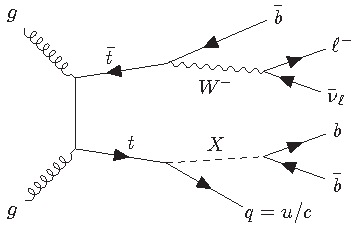
\includegraphics[width=0.47\textwidth]{TQX/diagramtXq.pdf}
    \caption{
        Leading-order Feynman diagram for the production and decay of a neutral scalar $X$ in a \ttbar\ event.
    }
    \label{tqx:feynman2}
    \end{center}
\end{figure}

The detector signature is defined to include exactly one isolated lepton $\ell$, considering only electrons and muons. Nonetheless, the $\tau$ leptons decaying into electrons or muons are included. As four quarks are present in the final state, four jets are expected to be reconstructed with at least three of them originating from a $b$-quark, and the last one as a $c$- or $u$-quark depending on the signal. The $b$-tagging is an important piece of the strategy as the selection of $t\to uX$ or $t\to cX$ signals will be affected by the different efficiencies of rejecting or accepting $c$- and $u$-quarks.\\

The  complexity of the targeted final state originates from the dominant \ttbar\ production with additional jets (\ttjets). In particular, \ttb\ is the main irreducible background while the \ttl\ background is reducible and can be suppressed by tightening the $b$-tagging selection\footnote{The rejection of light-quarks is three times larger from the 70\% to the 60\% working point with the DL1r algorithm.}. The correct modelling of \ttbar\ events is key for the analysis and unfortunately, the process is poorly constrained by data measurements,  and has large theory uncertainties.\\

\section{Event selection}
\label{tqX:SectionEventSelection}
This section describes the selection of the events used in the analysis, applied to data and simulated events. The physics objects are described in more detail in Chapter~\ref{chapter:EventReco}.\\

The full Run~2 data, recorded with the~\acrshort{ATLASlabel} detector at the~\acrshort{LHClabel} from $\sqrt{s}$=13~TeV $pp$ collisions for a total integrated luminosity of 139~fb$^{-1}$, is analysed. Events are required to be triggered by the single-lepton triggers, which are shared with the $H^+\to tb$ analysis (Section~\ref{Hplustb:SectionEventSelection}).\\

Multiple triggers are used in order to maximise the selection efficiency, either with low \pT\ thresholds and lepton identification and isolation requirements, or with higher thresholds but looser identification criteria and no isolation requirements. Slightly different sets of triggers are used for 2015 and 2016-2018 data due to the increase in pile-up. Furthermore, at least one primary vertex is required.\\ %The minimum \pT\ required by the triggers was increased to keep both trigger rate and data storage within their limits. For muons, the lowest \pT\ threshold was 20 (26) GeV in 2015 (2016-2018), while for electrons, triggers with a minimum \pT\ threshold of 24 (26) GeV were used [44 H+paper]. 

% \begin{table}[htbp]
%     \begin{tabular}{l|cccccc}
%     \toprule\toprule
%     \multirow{2}{*}{Object} & \multicolumn{2}{c}{\pT\ threshold [GeV]}    & \multicolumn{2}{c}{Identification} & \multicolumn{2}{c}{Isolation} \\    
%         & 2015       & 2016-2018    & 2015    & 2016-2018   & 2015   & 2016-2018   \\  \midrule \midrule
%         \multirow{3}{*}{Electron} & 24        & 26     & medium    & tight    & -   & loose   \\
%                                   & 60        & 60     & medium    & medium   & -   & -   \\
%                                   & 120       & 140    & loose     & loose    & -   & -   \\ \midrule
%         \multirow{2}{*}{Muons}    & 20        & 26     & medium    & medium    & loose   & medium   \\
%                                   & 50        & 50     & medium    & medium   & -   & -   \\
%         \bottomrule\bottomrule                               
%     \end{tabular}
%     \caption{Single-lepton triggers and quality criteria used for the $t\to qX$ analysis.}
%     \label{tqX:triggertable}
% \end{table}

Leptons are required to fulfil the \textit{tight} identification for electrons and \textit{medium} for muons. In addition, electrons are required to satisfy the \textit{tight} isolation criteria while muons are required the \textit{TightTrackOnly FixedRad} criteria. Hadronically decaying $\tau$ leptons are required to have $\pT>25$~GeV and pass the \textit{mediumRNN} identification working point, and are used for the object overlap removal.\\

PFlow jets are used with a radius parameter $R=0.4$. To reduce pile-up effects, the JVT algorithm is applied for jets with $\abs{\eta}<2.4$ and $\pT<60$~GeV.% algorithm that matches jets with pT < 120 GeV and |η| < 2.4 to tracks with pT > 0.4 GeV to identify jets consistent with the primary vertex. This algorithm is known as jet vertex tagger (JVT) [80]
The $b$-jets are identified and selected using the 70\% working point of the DL1r tagger. Jets that pass the 70\% working point but not the 60\% are referred to as $bl$-jets (for $loose$ $b$-tagging). The pseudo-continuous score of the different jets is used in the analysis.\\

Events are required to have at least four jets, at least two of which are required to be tagged with the 60\% $b$-tagging working point and one additional one fulfilling the 70\% ($bl$) working point. In addition, exactly one lepton with $\pT>27$~GeV and no additional lepton with $\pT>10$~GeV passing the \textit{medium} (\textit{loose}) identification working point for electrons (muons) is required. Further requirements on \MET\ and the transverse mass of the lepton and \MET\ ($m_{\text{T}}^W$) are applied for both muon and electron channels to further reject multi-jet background: $\MET\geq20$~GeV and $\MET+m_{\text{T}}^W\geq60$~GeV.\\

\section{Signal and background modelling}

The final state of the signal consists of three $b$-jets, one light-jet from either a $c$- or $u$-quark, one lepton and one neutrino. Such final state is shared fully or partially by a large number of background processes, the main one being \ttjets. Additional contributions to the background are from the production of $W$ and $Z$ bosons with jets ($V$+jets), single-top-quark production, diboson processes ($VV$) and the associated production of bosons and top quarks ($\ttbar V$, $\ttbar H$). Non-prompt leptons and misidentified jets form what is known as multi-jet background, whose contribution is negligible due to the trigger and lepton quality requirements.\\

Compared to the $H^+\to tb$ search, the final state is very similar and the same simulated background can be used, detailed in Section~\ref{Hplustb:Sectionmodelling}. The main difference is the treatment of the small background, as the selection is tighter; and the increased relevance of the \ttbar\ background events with the $W\to cb$ decay allowed, due to the presence of a $c$-quark in the $t\to cX$ signal.\\

%Various \acrshort{MClabel} generators have been used for the production of the samples. Table~\ref{tqX:MCsummarytable} lists all simulated samples used in the analysis, both nominal which are use for the baseline~\acrshort{SMlabel} background prediction and the alternative samples, used primarily to estimate systematic uncertainties. In general, the settings described in \textcolor{red}{Section} apply for the generated samples. Also, the detector response is simulated either with \GEANT~4 or AF-II for the full detector or the fast simulation. The pile-up interactions are simulated with \PYTHIA~8 and events are weighted to match the respective pile-up profiles observed in data during Run~2 (average of 34 interactions).%If not stated otherwise, the~\acrshort{MElabel} generator is used at NLO with the \textit{NNPDF3.0NLO}~\acrshort{PDFlabel} set for 5FS samples and the \textit{NNPDF3.0NLOf4} for the 4FS samples

% \begin{table}[htbp]
%     \scriptsize	
%     \addtolength{\leftskip} {-2cm} % menja marges
%     \addtolength{\rightskip}{-2cm}
%     \begin{tabular}{llllll}
%     \toprule\toprule
%     Process & ME generator & PS generator &  Normalisation & PDF set & Simulation \\ \midrule \midrule
%     $t\to qX$             & \MGMCatNLO~2.6.2    & \PYTHIA~8.244    & NLO   & \textit{NNPDF2.3NLO}   & Fast   \\  \midrule \midrule
%     \multicolumn{2}{l}{\ttbar and single-top}  &  &  &  &  \\ \midrule 
%     \ttbar                & \POWHEGBOX~v2 & \PYTHIA~8.230    & NNLO+NNLL   & \textit{NNPDF3.0NLO}   & Fast   \\ 
%                           & \POWHEGBOX~v2 & \HERWIG~7.04     & NNLO+NNLL   & \textit{NNPDF3.0NLO}   & Fast   \\ 
%     \ttbar+\bbar (4FS)    & \textsc{PowhegBoxRes} & \PYTHIA~8.230    & NNLO+NNLL   & \textit{NNPDF3.0NLOnf4}   & Fast   \\ 
%     $Wt$                  & \POWHEGBOX~v2 (DR) & \PYTHIA~8.230  & NNLO+NNLL   & \textit{NNPDF3.0NLO}   & Full/Fast \\ 
%                           & \POWHEGBOX~v2 (DS) & \PYTHIA~8.230  & NNLO+NNLL   & \textit{NNPDF3.0NLO}   & Full \\ 
%                           & \POWHEGBOX~v2 (DR) & \HERWIG~7.04   & NNLO+NNLL   & \textit{NNPDF3.0NLO}   & Fast \\ 
%                           & \MGMCatNLO~2.6.2 (DR) & \PYTHIA~8.230  & NNLO+NNLL   & \textit{CT10NLO}   & Fast \\ 
%     $t$-channel           & \POWHEGBOX~v2    & \PYTHIA~8.230  & NLO   & \textit{NNPDF3.0NLOnf4}   & Full \\ 
%                           & \POWHEGBOX~v2    & \HERWIG~7.04   & NLO   & \textit{NNPDF3.0NLOnf4}   & Fast? \\ 
%                           & \MGMCatNLO~2.6.2 & \PYTHIA~8.230  & NLO   & \textit{NNPDF3.0NLOnf4}   & Fast? \\ 
%     $s$-channel           & \POWHEGBOX~v2    & \PYTHIA~8.230  & NLO   & \textit{NNPDF3.0NLO}      & Full \\ 
%                           & \POWHEGBOX~v2    & \HERWIG~7.04   & NLO   & \textit{NNPDF3.0NLO}      & Fast? \\ 
%                           & \MGMCatNLO~2.6.2 & \PYTHIA~8.230  & NLO   & \textit{NNPDF3.0NLO}      & Fast? \\ 
%     \midrule \midrule
%     $V$+jets &  &  &  &  &  \\ \midrule 
%     $W$+jets & \SHERPA~v2.2.1 (2j@NLO, 4j@LO) & \SHERPA & NNLO & \textit{NNPDF3.0NNLO} & Full \\
%     $Z$+jets & \SHERPA~v2.2.1 (2j@NLO, 4j@LO) & \SHERPA & NNLO & \textit{NNPDF3.0NNLO} & Full \\    
%     \midrule \midrule
%     Diboson &  &  &  &  &  \\ \midrule 
%     $VV$ (had.)    & \SHERPA~v2.2.1 & \SHERPA & NLO & \textit{NNPDF3.0NNLO} & Full \\
%     $VV$ (lep.)    & \SHERPA~v2.2.2 & \SHERPA & NLO & \textit{NNPDF3.0NNLO} & Full \\
%     $VV$ (lep.+jj) & \SHERPA~v2.2.2 (EW@NLO) & \SHERPA & NLO & \textit{NNPDF3.0NNLO} & Full \\
%     \midrule \midrule
%     $\ttbar+V$ &  &  &  &  &  \\ \midrule    
%     $\ttbar W$         & \MGMCatNLO~v2.3.3      & \PYTHIA~8.210 & NLO+NLO (EW) & \textit{NNPDF3.0NLO} & Full \\
%                        & \SHERPA~v2.0.0 (2j@LO) & \SHERPA       & NLO+NLO (EW) & \textit{NNPDF3.0NNLO} & Full \\
%     $\ttbar\ell\ell$   & \MGMCatNLO~v2.3.3      & \PYTHIA~8.210 & NLO+NLO (EW) & \textit{NNPDF3.0NLO} & Full \\
%                        & \SHERPA~v2.0.0 (1j@LO) & \SHERPA       & NLO+NLO (EW) & \textit{NNPDF3.0NNLO} & Full \\
%     $\ttbar Z$ ($qq$, $\nu\nu$) & \MGMCatNLO~v2.3.3 & \PYTHIA~8.210 & NLO+NLO (EW) & \textit{NNPDF3.0NLO} & Full \\
%                        &\SHERPA~v2.0.0 (2j@LO) & \SHERPA       & NLO+NLO (EW) & \textit{NNPDF3.0NNLO} & Full \\    
%     \midrule \midrule
%     Others &  &  &  &  &  \\ \midrule
%     \ttbar\ttbar & \MGMCatNLO~v2.3.3       & \PYTHIA~8.230  & NLO+NLO (EW)  & \textit{NNPDF3.1NLO} & Full \\
%     $tZq$        & \MGMCatNLO~v2.3.3  & \PYTHIA~8.212  & NLO           & \textit{CTEQ6L1} & Full \\
%     $tWZ$        & \MGMCatNLO~v2.3.3 (DR)  & \PYTHIA~\textcolor{red}{8.212} & NLO  & \textit{NNPDF3.0NLO} & Full \\
%     $\ttbar H$   & \POWHEGBOX~v2 & \PYTHIA~8.230 & NLO+NLO (EW) & \textit{NNPDF3.0NLO} & Full/Fast \\
%                  & \POWHEGBOX~v2 & \HERWIG~7.04  & NLO+NLO (EW) & \textit{NNPDF3.0NLO} & Fast \\
%                  & \MGMCatNLO~v2.6.0      & PYTHIA8.230     & NLO+NLO (EW) & \textit{NNPDF3.0NLO}    & Fast \\
%     $tHjb$       & \MGMCatNLO~v2.6.2      & PYTHIA8.230     & NLO          & \textit{NNPDF3.0NLOnf4} & Full \\
%     $tWH$        & \MGMCatNLO~v2.6.2 (DR) &  PYTHIA8.235    & NLO          & \textit{NNPDF3.0NLO}    & Full \\

%     \bottomrule\bottomrule                               
%     \end{tabular}
%     \caption{Summary of all simulated \acrshort{MClabel} samples used in the $t\to qX$ analysis. The nominal sample is the first row for each process. DR and DS stand for the diagram removal scheme \textcolor{red}{229} and the diagram
%     subtraction scheme 170, 229, respectively.}
%     \label{tqX:MCsummarytable}
% \end{table}
% %https://iopscience.iop.org/article/10.1088/1126-6708/2008/07/029
% %https://cds.cern.ch/record/2216168


\subsection{Signal modelling}

The signal of this analysis is a \ttbar\ event with one top decaying $t\to qX$ with $X\to\bbar$ and $q=u,c$. The samples are generated with \POWHEGBOX~v2 interfaced with \MADSPIN and \PYTHIA~8.2. The \ttbar\ production is modelled at NLO with the \textit{NNPDF2.3NLO}~\acrshort{PDFlabel} set. The top-quark decays are modelled in \MADSPIN both the $t\to Wb$ and $t\to qX$ decays, assuming a neutral spin-0 scalar $X$ based on the LO \textit{NNPDF2.3}  model with B$(X\to\bbar)=100\%$ and the decay width set to 0.4~MeV (same as the \acrshort{SMlabel} Higgs). The events are showered with \PYTHIA~8.244.\\

A total of fifty-two samples are generated corresponding to thirteen different values of $m_X$ ranging from 20 to 160~GeV and four different decays: $t\to uX$, $\bar{t}\to \bar{u}X$, $t\to cX$ and $\bar{t}\to \bar{c}X$. Table~\ref{tqX:signalsummarytable} lists the different mass-points and the number of events generated across the different decays.\\

\begin{table}[htbp]
    \small	
    \begin{tabular}{cc}
    \toprule\toprule
    $m_X$ [GeV] & Generated \\ \midrule
    20  & 1.50M \\
    30  & 1.49M \\
    40  & 1.50M \\
    50  & 1.50M \\
    60  & 1.50M \\
    70  & 1.49M \\
    80  & 1.50M \\
    90  & 1.50M \\
    100 & 1.50M \\
    120 & 1.50M \\
    140 & 1.50M \\
    150 & 1.50M \\
    160 & 1.50M \\

    \bottomrule\bottomrule  
    \end{tabular}                            
    \caption{Summary of the generated events for the different $t\to qX$ signal samples with different mass hypotheses, $m_X$.}
    \label{tqX:signalsummarytable}
\end{table}

\clearpage

% \subsection{Background modelling}

% \subsubsection{\ttbar+ jets}

% The dominant background for the $t\to qX$ signal is the \ttbar\ pair production with additional jets, especially \ttb\ processes. Hence, events are categorised depending on the flavour of the additional jets. The labelling is performed with \textit{particle jets}, jets formed only taking account particles with a mean lifetime over $3\cdot10^{-11}$~s not originating directly from top-quarks or $W$-bosons. Then, the jet flavour label is assigned from $\Delta R$(jet,hadron)<0.4 as follows:
% \begin{itemize}
%     \item \ttb: \ttbar + at least one additional jet containing at least one $b$-hadron.
%     \item \ttc: not \ttb\ and at least one additional jet containing at least one $c$-hadron.
%     \item \ttl: all other cases.
% \end{itemize}

% The nominal production is modelled with the 5FS and \POWHEGBOX~v2 setting the renormalisation and factorisation scales to $µ_R = µ_F = m_\text{T}$(top) and $h_\text{damp}=1.5\cdot m_\text{top}$. The parton shower and hadronisation processes are simulated with \PYTHIA~8. All \todo{only from tqX}generated \ttbar\ samples assume a diagonal Cabibbo-Kobayashi-Maskawa matrix, thus the $W\to cb$ contribution is not included $(B = 5.72 \times 10^{-4}$. Additional \ttjets\ events are produced with one of the $W$-bosons decaying leptonically and the other to $cb$, using the \acrshort{SMlabel} with non-zero Wolfenstein coefficients and 5FS.

% \subsubsection{Single-top}
% \textit{t-channel}

% Single-top t-channel production is modelled with \POWHEGBOX~v2, which provides~\acrshort{MElabel} at NLO in the 4FS with the \textit{NNPDF3.0NLOnf4}~\acrshort{PDFlabel} set. The renormalisation and factorisation scales are set to $µ_F=µ_R=\sqrt{m_b^2+p_{\text{T},b}^2}$. The events are showered with \PYTHIA~8.
% %The impact of the PS and hadronisation model is evaluated by comparing the nominal generator setup with a
% %sample produced with the PowhegBox v2 generator at NLO in QCD in the 4FS using the NNPDF3.0NLOnf4
% %PDF set. The same events produced for the nominal PowhegBox+Pythia8 sample are used. The events are
% %showered with Herwig 7.04.
% %To assess the uncertainty due to the choice of the matching scheme, the nominal sample is compared
% %to a sample generated with the MG5_aMC v2.6.2 generator at NLO in QCD in the 4FS, using the
% %NNPDF3.0NLOnf4 PDF set. Top quarks are decayed at LO using MadSpin [56, 57] to preserve all spin
% %correlations. The events are showered with Pythia 8.230.

% \textit{s-channel}

% Single-top s-channel production is modelled using the \POWHEGBOX~v2, which provides~\acrshort{MElabel} at NLO in the 5FS scheme with the \textit{NNPDF3.0NLO}~\acrshort{PDFlabel} set. The renormalisation and factorisation scales are set to the top-quark mass. The events are showered with \PYTHIA~8.
% %The impact of the PS and hadronisation model is evaluated by comparing the nominal generator setup with
% %a sample produced with the PowhegBox v2 generator at NLO in QCD in the 5Fs using the NNPDF3.0NLO
% %PDF set. The same events produced for the nominal PowhegBox+Pythia8 sample are used. The events are
% %showered with Herwig 7.04.
% %To assess the uncertainty due to the choice of the matching scheme, the nominal sample is compared
% %to a sample generated with the MG5_aMC v2.6.2 generator at NLO in QCD in the 5FS, using the
% %NNPDF3.0NLO PDF set. Top quarks are decayed at LO using MadSpin to preserve all spin correlations.
% %The events are showered with Pythia 8.230.

% \textit{$Wt$}

% Single-top $Wt$ associated production is modelled using \POWHEGBOX~v2, which provides~\acrshort{MElabel} at NLO in the 5FS with the \textit{NNPDF3.0NLO}~\acrshort{PDFlabel} set. The renormalisation and factorisation scales are set to the top-quark mass. The diagram removal scheme is employed to handle the interference with \ttbar\ production. %https://cds.cern.ch/record/2216168 https://iopscience.iop.org/article/10.1088/1126-6708/2008/07/029
% The events are showered with \PYTHIA~8.
% %The nominal Powheg+Pythia8 sample is compared to an alternative sample generated using the diagram
% %subtraction scheme [46, 58] to estimate the uncertainty due to the interference with tt¯ production.
% %The impact of the PS and hadronisation model is evaluated by comparing the nominal generator setup with
% %a sample produced with the Powheg v2 generator at NLO in QCD in the 5FS using the NNPDF3.0NLO
% %PDF set. The same events produced for the nominal Powheg+Pythia8 sample are used. The events are
% %showered with Herwig7.04.
% %To assess the uncertainty due to the choice of the matching scheme, the nominal sample is compared
% %to a sample generated with the MG5_aMC v2.6.2 generator at NLO in QCD in the 5FS, using the
% %NNPDF2.3NLO PDF set. The events are showered with Pythia 8.230.

% \subsubsection{$\ttbar+V$}
% The production of $\ttbar+V$ events is modelled using \MGMCatNLO~v2.3.3, which provides~\acrshort{MElabel} at NLO with the \textit{NNPDF3.0NLO}~\acrshort{PDFlabel} set. The renormalisation and factorisation scales are set to $\frac{1}{2}\sum_i\sqrt{m(i)^2+\pT(i)^2}$, where $i$ runs over the final-state particles used in the generation. The events are showered with \PYTHIA~8.
% %Additional ttV¯ samples are produced with the Sherpa 2.2.0 [52] generator at LO accuracy, using the
% %MEPS@LO setup [53, 54] with up to one additional parton for the ttV¯ sample and two additional partons
% %for the others. A dynamic µr is used, defined similarly to that of the nominal MG5_aMC+Pythia samples.
% %The CKKW matching scale of the additional emissions is set to 30 GeV. The default Sherpa 2.2.0 PS is
% %used along with the NNPDF3.0NNLO PDF set.

% \subsubsection{$V+jets$}
% Vector bosons plus jets production is simulated with the \SHERPA~v2.2.1 generator. In this setup, NLO-accurate \acrshort{MElabel} for up to two jets, and LO-accurate \acrshort{MElabel} for up to four jets are calculated with the Comix [62] and OpenLoops [63, 64] libraries. %https://iopscience.iop.org/article/10.1088/1126-6708/2008/12/039 ; https://journals.aps.org/prl/abstract/10.1103/PhysRevLett.108.111601 https://www.sciencedirect.com/science/article/abs/pii/S0010465516303320?via%3Dihub
% The default Sherpa PS %https://iopscience.iop.org/article/10.1088/1126-6708/2008/03/038
% based on Catani-Seymour dipoles and the cluster hadronisation model are used. They employ the dedicated set of tuned parameters developed by the Sherpa authors for this version, based on the \textit{NNPDF3.0nnlo} \acrshort{PDFlabel} set. %The NLO ME of a given jet- productioplicity are matched to the PS using a colour-exact variant of the MC@NLO algorithm [67].
% %Different jet multiplicities are then merged into an inclusive sample using an improved CKKW matching
% %procedure [53, 54], which is extended to NLO accuracy using the MEPS@NLO prescription [68]. The
% %merging cut is set to Qcut = 20 GeV.
% %QCD scale uncertainties have been evaluated on-the-fly [69] using 7-point variations of µf and µr in
% %the ME. The scales are varied independently by factors of 0.5 and 2 but avoiding opposite factors. PDF
% %uncertainties for the nominal PDF set are evaluated using the 100 variation replicas, as well as ±0.001
% %shifts of αS.

% \subsubsection{Diboson}
% Diboson samples are simulated with the \SHERPA~v2.2 generator. In this setup multiple \acrshort{MElabel} are matched and merged with the \SHERPA PS based on Catani-Seymour dipole using the MEPS@NLO prescription. For semi-leptonically and fully leptonically decaying diboson samples, as well as loop-induced diboson samples, the virtual QCD correction for \acrshort{MElabel} at NLO accuracy are provided by the OpenLoops library. For electroweak $VVjj$ production, the calculation is performed in the $G_\mu$ scheme, ensuring an optimal description of pure electroweak interactions at the electroweak scale. All samples are generated using the \textit{NNPDF3.0nnlo} set, along with the dedicated set of tuned PS parameters.

% \subsubsection{Other small background}

% \textit{$\ttbar H$}

% The production of $\ttbar H$ events is modelled with the \POWHEGBOX generator at NLO in the 5FS with the \textit{NNPDF3.0NLO} \acrshort{PDFlabel} set. The $h_\text{damp}$ parameter is set to $\frac{3}{4}\cdot(m_t + m_{tbar} + m_H ) = 352.5$~GeV. The events are showered with \PYTHIA~8.% The uncertainties due to ISR, FSR, PS and hadronisation
% %model, as well as that due to the matching scheme, are evaluated with the same procedures used for the tt¯ +
% %jets background.

% \textit{$tH$}

% The production of $tHjb$ events is modelled using the \MGMCatNLO~v2.6.0 generator in the 4FS with the \textit{NNPDF3.0NLOnf4} \acrshort{PDFlabel} set. The renormalisation and factorisation scales are set to $\frac{1}{2}\sum_i\sqrt{m(i)^2+\pT(i)^2}$, where $i$ runs over the final-state particles used in the generation. The shower starting scale is set to $\mu_q = \HT /2$, where \HT\ is defined as the scalar sum of the \pT\
% of all outgoing partons. The events are showered with \PYTHIA~8.230.

% The production of $tHW$ events is modelled instead using the \MGMCatNLO~v2.6.2 generator in the 5FS with the \textit{NNPDF3.0NLO} \acrshort{PDFlabel} set. The different scales are set to the same forms as for $tH$. The events are showered with \PYTHIA~8.235.

% \textit{$t\bar{t}t\bar{t}$}

% The production of four tops events is modelled using the \MGMCatNLO~v2.3.3 generator, which provides \acrshort{MElabel} at NLO with the \textit{NNPDF3.1NLO} \acrshort{PDFlabel} set. The renormalisation and factorisation scales are set to $\frac{1}{2}\sum_i\sqrt{m(i)^2+\pT(i)^2}$, where $i$ runs over the final-state particles used in the generation. The events are showered with \PYTHIA~8.230.\todo{I dont think these are included.}

% \textit{$tZq$ and $tZW$}

% The $tZq$ events are generated using the \MGMCatNLO~v2.3.3 generator at LO in the 4FS with the \textit{CTEQ6L1} LO \acrshort{PDFlabel} set. The renormalisation and factorisation scales are set to $4\sqrt{m(b)^2+\pT(b)^2}$, where the $b$-quark comes from the gluon splitting.

% The $tZW$ sample is simulated using the \MGMCatNLO~v2.3.3 generator but at NLO in the 5FS with the \textit{NNPDF3.0NLO} \acrshort{PDFlabel} set. The top quark is decayed inclusively while the Z boson decays to a pair of leptons. he renormalisation and factorisation scales are set instead to the top quark mass. The DR scheme is applied to handle the interference with $ttZ$.

% %Both $tZq$ and $tZW$ are showered with \PYTHIA~8.212.